\documentclass[12pt]{article}
\usepackage{tikz}
\usepackage{amsmath}
% Underlining package
\usepackage{ulem}
\usetikzlibrary{calc}
\usetikzlibrary{angles,quotes}
\usepackage[a4paper, portrait, margin=1cm]{geometry}
\usepackage{fancyhdr}

\newcommand{\HeadingAnswers}{%
\section*{\Large Name: \underline{\hspace{8cm}} \hfill Date: \underline{\hspace{3cm}}}%
\vspace{-3mm}\par
\textbf{Volume of a Rectangular Prism: Answers}\vspace{1pt}\hrule
}

% raise footer with page number; no header
\fancypagestyle{myfancypagestyle}{
  \fancyhf{}% clear all header and footer fields
  \renewcommand{\headrulewidth}{0pt} % no rule under header
  \fancyfoot[C] {\thepage} \setlength{\footskip}{14.5pt} % raise page number allowed min 14.5pt
}
\pagestyle{myfancypagestyle}  % apply myfancypagestyle

\newif\ifTrue
\newif\ifFalse

\Truetrue   % Enables \ifTrue
\Falsefalse % Enables \ifFalse

\newcounter{minipagecount}

\begin{document}
\HeadingAnswers
\vspace{8mm}

\begin{minipage}{0.55\textwidth}
  \refstepcounter{minipagecount}
  \noindent{(\theminipagecount)}\quad
  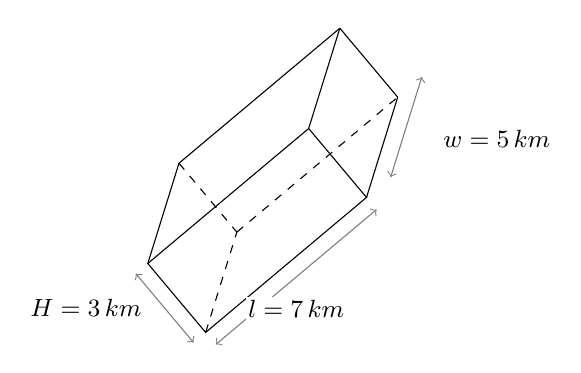
\begin{tikzpicture}[scale=1.0, baseline=(current bounding box.north)]
    \begin{scope}[rotate=40]

        % front face
        \coordinate (K) at (0,0);
        \coordinate (L) at (2.667,0);
        \coordinate (M) at (2.667,1.143);
        \coordinate (N) at (0,1.143);

        % back face skew shift
        \coordinate (Q) at ($(K)+(1.122, 0.721)$);
        \coordinate (R) at ($(L)+(1.122, 0.721)$);
        \coordinate (S) at ($(M)+(1.122, 0.721)$);
        \coordinate (T) at ($(N)+(1.122, 0.721)$);

        % draw prism edges
        \draw[] (K)--(L)--(M)--(N)--cycle;
        \draw[dashed] (K)--(Q);
        \draw[] (L)--(R);
        \draw[] (M)--(S);
        \draw[] (N)--(T);
        \draw[dashed] (Q)--(R);
        \draw[] (R)--(S);
        \draw[] (S)--(T);
        \draw[dashed] (T)--(Q);

        % Vertex LABELS
        % Labels relative to shape geometry
        % \ifTrue  or \ifFalse
        \ifTrue
            % \node at ($(K)+(-0.2,-0.2)$) {K};
            % \node at ($(L)+(0.2,-0.2)$) {L};
            % \node at ($(M)+(0.2,0.2)$) {M};
            % \node at ($(N)+(-0.2,0.2)$) {N};
            \node[above left] at (K) {K};
            \node[below right] at (L) {L};
            \node[above right] at (M) {M};
            \node[above left] at (N) {N};
            \node[below left] at (Q) {Q};
            \node[below right] at (R) {R};
            \node[above right] at (S) {S};
            \node[above left] at (T) {T};
        \fi


       % dimension lines enabled
        \draw[<->, gray]
            ($(K) + (0,-0.2)$) -- ($(L) + (0,-0.2)$)
            node[black, midway, fill=white, fill opacity=1.0, text opacity=1, inner sep=1pt, shift={(0,-0.4)}]
            {\small $l = 7\,km$};

        \draw[<->, gray]
            ($(K) + (-0.2,0)$) -- ($(N) + (-0.2,0)$)
            node[black, midway, fill=white, fill opacity=1.0, text opacity=1, inner sep=1pt, shift={(-1.0,0)}]
            {\small $H=3\,km$};


        \draw[<->, gray]
            ($(L) + (0.4,0)$) -- ($(R) + (0.4,0)$)
            node[black, midway, fill=white, fill opacity=1.0, text opacity=1, inner sep=1pt, shift={(1.15,-0.15)}]
            {\small $w=5\,km$};


        % dimension lines enabled
        % \coordinate (P1offAB) at ($ (K)+(0,-0.2) $);
        % \coordinate (P2offAB) at ($ (L)+(0,-0.2) $);
        % \draw[<->, gray] (P1offAB)--(P2offAB);
        % \node[black, fill=white, fill opacity=1.0, text opacity=1, inner sep=1pt]
        %     at ($ (P1offAB)!0.5!(P2offAB) + (0,-0.4) $) {\small $l=7 km$};


        % \coordinate (P1offAD) at ($ (K)+(-0.2,0) $);
        % \coordinate (P2offAD) at ($ (N)+(-0.2,0) $);
        % \draw[<->, gray] (P1offAD)--(P2offAD);
        % \node[black, fill=white, fill opacity=1.0, text opacity=1, inner sep=1pt]
        %     at ($ (P1offAD)!0.5!(P2offAD) + (-1.0,0) $) {\small $H=3 km$};

        % \coordinate (P1offBF) at ($ (L)+(0.4,0) $);
        % \coordinate (P2offBF) at ($ (R)+(0.4,0) $);
        % \draw[<->, gray] (P1offBF)--(P2offBF);
        % \node[black, fill=white, fill opacity=1.0, text opacity=1, inner sep=1pt]
        %     at ($ (P1offBF)!0.5!(P2offBF) + (1.15,-0.15) $) {\small $w=5 km$};

    \end{scope}
\end{tikzpicture}
\end{minipage}%
\hfill
\begin{minipage}{.4\textwidth}
  \begin{align*}
    \text{Volume} &= lwH \\
    \text{Volume} &= 7 \,\text{<<calc_units>>} \times 5 \,\text{<<calc_units>>} \times 3 \,\text{<<calc_units>>} \\
    \text{Volume} &= 105 \,\text{<<calc_units>>}^2
  \end{align*}
\end{minipage}

\vspace{1cm} \vfill\begin{minipage}{0.55\textwidth}
  \refstepcounter{minipagecount}
  \noindent{(\theminipagecount)}\quad
  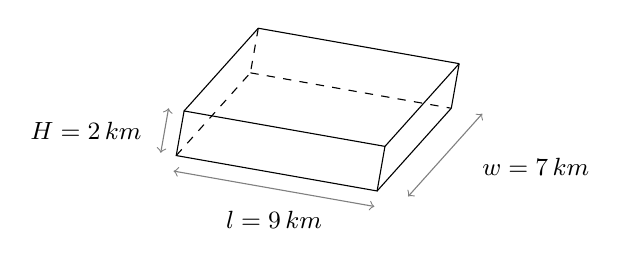
\begin{tikzpicture}[scale=1.0, baseline=(current bounding box.north)]
    \begin{scope}[rotate=-10]

        % front face
        \coordinate (Q) at (0,0);
        \coordinate (R) at (2.59,0);
        \coordinate (S) at (2.59,0.575);
        \coordinate (T) at (0,0.575);

        % back face skew shift
        \coordinate (W) at ($(Q)+(0.745, 1.198)$);
        \coordinate (X) at ($(R)+(0.745, 1.198)$);
        \coordinate (Y) at ($(S)+(0.745, 1.198)$);
        \coordinate (Z) at ($(T)+(0.745, 1.198)$);

        % draw prism edges
        \draw[] (Q)--(R)--(S)--(T)--cycle;
        \draw[dashed] (Q)--(W);
        \draw[] (R)--(X);
        \draw[] (S)--(Y);
        \draw[] (T)--(Z);
        \draw[dashed] (W)--(X);
        \draw[] (X)--(Y);
        \draw[] (Y)--(Z);
        \draw[dashed] (Z)--(W);

        % Vertex LABELS
        % Labels relative to shape geometry
        % \ifTrue  or \ifFalse
        \ifTrue
            % \node at ($(Q)+(-0.2,-0.2)$) {Q};
            % \node at ($(R)+(0.2,-0.2)$) {R};
            % \node at ($(S)+(0.2,0.2)$) {S};
            % \node at ($(T)+(-0.2,0.2)$) {T};
            \node[above left] at (Q) {Q};
            \node[below right] at (R) {R};
            \node[above right] at (S) {S};
            \node[above left] at (T) {T};
            \node[below left] at (W) {W};
            \node[below right] at (X) {X};
            \node[above right] at (Y) {Y};
            \node[above left] at (Z) {Z};
        \fi


       % dimension lines enabled
        \draw[<->, gray]
            ($(Q) + (0,-0.2)$) -- ($(R) + (0,-0.2)$)
            node[black, midway, fill=white, fill opacity=1.0, text opacity=1, inner sep=1pt, shift={(0,-0.4)}]
            {\small $l = 9\,km$};

        \draw[<->, gray]
            ($(Q) + (-0.2,0)$) -- ($(T) + (-0.2,0)$)
            node[black, midway, fill=white, fill opacity=1.0, text opacity=1, inner sep=1pt, shift={(-1.0,0)}]
            {\small $H=2\,km$};


        \draw[<->, gray]
            ($(R) + (0.4,0)$) -- ($(X) + (0.4,0)$)
            node[black, midway, fill=white, fill opacity=1.0, text opacity=1, inner sep=1pt, shift={(1.15,-0.15)}]
            {\small $w=7\,km$};


        % dimension lines enabled
        % \coordinate (P1offAB) at ($ (Q)+(0,-0.2) $);
        % \coordinate (P2offAB) at ($ (R)+(0,-0.2) $);
        % \draw[<->, gray] (P1offAB)--(P2offAB);
        % \node[black, fill=white, fill opacity=1.0, text opacity=1, inner sep=1pt]
        %     at ($ (P1offAB)!0.5!(P2offAB) + (0,-0.4) $) {\small $l=9 km$};


        % \coordinate (P1offAD) at ($ (Q)+(-0.2,0) $);
        % \coordinate (P2offAD) at ($ (T)+(-0.2,0) $);
        % \draw[<->, gray] (P1offAD)--(P2offAD);
        % \node[black, fill=white, fill opacity=1.0, text opacity=1, inner sep=1pt]
        %     at ($ (P1offAD)!0.5!(P2offAD) + (-1.0,0) $) {\small $H=2 km$};

        % \coordinate (P1offBF) at ($ (R)+(0.4,0) $);
        % \coordinate (P2offBF) at ($ (X)+(0.4,0) $);
        % \draw[<->, gray] (P1offBF)--(P2offBF);
        % \node[black, fill=white, fill opacity=1.0, text opacity=1, inner sep=1pt]
        %     at ($ (P1offBF)!0.5!(P2offBF) + (1.15,-0.15) $) {\small $w=7 km$};

    \end{scope}
\end{tikzpicture}
\end{minipage}%
\hfill
\begin{minipage}{.4\textwidth}
  \begin{align*}
    \text{Volume} &= lwH \\
    \text{Volume} &= 9 \,\text{<<calc_units>>} \times 7 \,\text{<<calc_units>>} \times 2 \,\text{<<calc_units>>} \\
    \text{Volume} &= 126 \,\text{<<calc_units>>}^2
  \end{align*}
\end{minipage}

\vspace{1cm} \vfill\begin{minipage}{0.55\textwidth}
  \refstepcounter{minipagecount}
  \noindent{(\theminipagecount)}\quad
  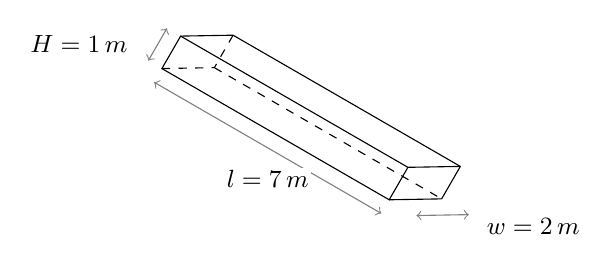
\begin{tikzpicture}[scale=1.0, baseline=(current bounding box.north)]
    \begin{scope}[rotate=-30]

        % front face
        \coordinate (A) at (0,0);
        \coordinate (B) at (3.333,0);
        \coordinate (C) at (3.333,0.476);
        \coordinate (D) at (0,0.476);

        % back face skew shift
        \coordinate (E) at ($(A)+(0.571, 0.343)$);
        \coordinate (F) at ($(B)+(0.571, 0.343)$);
        \coordinate (G) at ($(C)+(0.571, 0.343)$);
        \coordinate (H) at ($(D)+(0.571, 0.343)$);

        % draw prism edges
        \draw[] (A)--(B)--(C)--(D)--cycle;
        \draw[dashed] (A)--(E);
        \draw[] (B)--(F);
        \draw[] (C)--(G);
        \draw[] (D)--(H);
        \draw[dashed] (E)--(F);
        \draw[] (F)--(G);
        \draw[] (G)--(H);
        \draw[dashed] (H)--(E);

        % Vertex LABELS
        % Labels relative to shape geometry
        % \ifTrue  or \ifFalse
        \ifTrue
            % \node at ($(A)+(-0.2,-0.2)$) {A};
            % \node at ($(B)+(0.2,-0.2)$) {B};
            % \node at ($(C)+(0.2,0.2)$) {C};
            % \node at ($(D)+(-0.2,0.2)$) {D};
            \node[above left] at (A) {A};
            \node[below right] at (B) {B};
            \node[above right] at (C) {C};
            \node[above left] at (D) {D};
            \node[below left] at (E) {E};
            \node[below right] at (F) {F};
            \node[above right] at (G) {G};
            \node[above left] at (H) {H};
        \fi


       % dimension lines enabled
        \draw[<->, gray]
            ($(A) + (0,-0.2)$) -- ($(B) + (0,-0.2)$)
            node[black, midway, fill=white, fill opacity=1.0, text opacity=1, inner sep=1pt, shift={(0,-0.4)}]
            {\small $l = 7\,m$};

        \draw[<->, gray]
            ($(A) + (-0.2,0)$) -- ($(D) + (-0.2,0)$)
            node[black, midway, fill=white, fill opacity=1.0, text opacity=1, inner sep=1pt, shift={(-1.0,0)}]
            {\small $H=1\,m$};


        \draw[<->, gray]
            ($(B) + (0.4,0)$) -- ($(F) + (0.4,0)$)
            node[black, midway, fill=white, fill opacity=1.0, text opacity=1, inner sep=1pt, shift={(1.15,-0.15)}]
            {\small $w=2\,m$};


        % dimension lines enabled
        % \coordinate (P1offAB) at ($ (A)+(0,-0.2) $);
        % \coordinate (P2offAB) at ($ (B)+(0,-0.2) $);
        % \draw[<->, gray] (P1offAB)--(P2offAB);
        % \node[black, fill=white, fill opacity=1.0, text opacity=1, inner sep=1pt]
        %     at ($ (P1offAB)!0.5!(P2offAB) + (0,-0.4) $) {\small $l=7 m$};


        % \coordinate (P1offAD) at ($ (A)+(-0.2,0) $);
        % \coordinate (P2offAD) at ($ (D)+(-0.2,0) $);
        % \draw[<->, gray] (P1offAD)--(P2offAD);
        % \node[black, fill=white, fill opacity=1.0, text opacity=1, inner sep=1pt]
        %     at ($ (P1offAD)!0.5!(P2offAD) + (-1.0,0) $) {\small $H=1 m$};

        % \coordinate (P1offBF) at ($ (B)+(0.4,0) $);
        % \coordinate (P2offBF) at ($ (F)+(0.4,0) $);
        % \draw[<->, gray] (P1offBF)--(P2offBF);
        % \node[black, fill=white, fill opacity=1.0, text opacity=1, inner sep=1pt]
        %     at ($ (P1offBF)!0.5!(P2offBF) + (1.15,-0.15) $) {\small $w=2 m$};

    \end{scope}
\end{tikzpicture}
\end{minipage}%
\hfill
\begin{minipage}{.4\textwidth}
  \begin{align*}
    \text{Volume} &= lwH \\
    \text{Volume} &= 7 \,\text{<<calc_units>>} \times 2 \,\text{<<calc_units>>} \times 1 \,\text{<<calc_units>>} \\
    \text{Volume} &= 14 \,\text{<<calc_units>>}^2
  \end{align*}
\end{minipage}

\vspace{1cm} \vfill\begin{minipage}{0.55\textwidth}
  \refstepcounter{minipagecount}
  \noindent{(\theminipagecount)}\quad
  \begin{tikzpicture}[scale=1.0, baseline=(current bounding box.north)]
    \begin{scope}[rotate=0]

        % front face
        \coordinate (Q) at (0,0);
        \coordinate (R) at (2.963,0);
        \coordinate (S) at (2.963,4.444);
        \coordinate (T) at (0,4.444);

        % back face skew shift
        \coordinate (W) at ($(Q)+(0.802, 0.657)$);
        \coordinate (X) at ($(R)+(0.802, 0.657)$);
        \coordinate (Y) at ($(S)+(0.802, 0.657)$);
        \coordinate (Z) at ($(T)+(0.802, 0.657)$);

        % draw prism edges
        \draw[] (Q)--(R)--(S)--(T)--cycle;
        \draw[dashed] (Q)--(W);
        \draw[] (R)--(X);
        \draw[] (S)--(Y);
        \draw[] (T)--(Z);
        \draw[dashed] (W)--(X);
        \draw[] (X)--(Y);
        \draw[] (Y)--(Z);
        \draw[dashed] (Z)--(W);

        % Vertex LABELS
        % Labels relative to shape geometry
        % \ifTrue  or \ifFalse
        \ifTrue
            % \node at ($(Q)+(-0.2,-0.2)$) {Q};
            % \node at ($(R)+(0.2,-0.2)$) {R};
            % \node at ($(S)+(0.2,0.2)$) {S};
            % \node at ($(T)+(-0.2,0.2)$) {T};
            \node[above left] at (Q) {Q};
            \node[below right] at (R) {R};
            \node[above right] at (S) {S};
            \node[above left] at (T) {T};
            \node[below left] at (W) {W};
            \node[below right] at (X) {X};
            \node[above right] at (Y) {Y};
            \node[above left] at (Z) {Z};
        \fi


       % dimension lines enabled
        \draw[<->, gray]
            ($(Q) + (0,-0.2)$) -- ($(R) + (0,-0.2)$)
            node[black, midway, fill=white, fill opacity=1.0, text opacity=1, inner sep=1pt, shift={(0,-0.4)}]
            {\small $l = 4\,cm$};

        \draw[<->, gray]
            ($(Q) + (-0.2,0)$) -- ($(T) + (-0.2,0)$)
            node[black, midway, fill=white, fill opacity=1.0, text opacity=1, inner sep=1pt, shift={(-1.0,0)}]
            {\small $H=6\,cm$};


        \draw[<->, gray]
            ($(R) + (0.4,0)$) -- ($(X) + (0.4,0)$)
            node[black, midway, fill=white, fill opacity=1.0, text opacity=1, inner sep=1pt, shift={(1.15,-0.15)}]
            {\small $w=2\,cm$};


        % dimension lines enabled
        % \coordinate (P1offAB) at ($ (Q)+(0,-0.2) $);
        % \coordinate (P2offAB) at ($ (R)+(0,-0.2) $);
        % \draw[<->, gray] (P1offAB)--(P2offAB);
        % \node[black, fill=white, fill opacity=1.0, text opacity=1, inner sep=1pt]
        %     at ($ (P1offAB)!0.5!(P2offAB) + (0,-0.4) $) {\small $l=4 cm$};


        % \coordinate (P1offAD) at ($ (Q)+(-0.2,0) $);
        % \coordinate (P2offAD) at ($ (T)+(-0.2,0) $);
        % \draw[<->, gray] (P1offAD)--(P2offAD);
        % \node[black, fill=white, fill opacity=1.0, text opacity=1, inner sep=1pt]
        %     at ($ (P1offAD)!0.5!(P2offAD) + (-1.0,0) $) {\small $H=6 cm$};

        % \coordinate (P1offBF) at ($ (R)+(0.4,0) $);
        % \coordinate (P2offBF) at ($ (X)+(0.4,0) $);
        % \draw[<->, gray] (P1offBF)--(P2offBF);
        % \node[black, fill=white, fill opacity=1.0, text opacity=1, inner sep=1pt]
        %     at ($ (P1offBF)!0.5!(P2offBF) + (1.15,-0.15) $) {\small $w=2 cm$};

    \end{scope}
\end{tikzpicture}
\end{minipage}%
\hfill
\begin{minipage}{.4\textwidth}
  \begin{align*}
    \text{Volume} &= lwH \\
    \text{Volume} &= 4 \,\text{<<calc_units>>} \times 2 \,\text{<<calc_units>>} \times 6 \,\text{<<calc_units>>} \\
    \text{Volume} &= 48 \,\text{<<calc_units>>}^2
  \end{align*}
\end{minipage}

\vspace{1cm} \vfill

\end{document}
